\chapter{Hurtownie danych}


Definicję Hurtowni Danych \ang{Data Warehouse}  przypisuje się Bill'owi Inmon'owi w 1992 roku.
Zgodnie z tą definicją Hurtownią danych jest bazą danych mającą następujące cztery cechy.

\begin{itemize}
 \item Zorientowaną na temat \ang{ Subject-oriented} -- dane są gromadzone 
        w~ściśle określonej dziedzinie, aby możliwe było zrobienie sensownego zestawienia danych.
        Nie są przechowywane działania czy operacje biznesowe. Hurtownia danych  ograniczona w firmie do jednego działu 
        lub wybranego obszaru (np. Biznesowego), jest określana jako lokalna hurtownia danych lub tematyczna hurtownia danych \ang{data mart} stanowiąca podzbiór hurtowni danych
 \item Nie ulotność \ang{Non-volatile} -- dane przechowywane w Hurtowni danych nie są nigdy usuwane i modyfikowane, 
        przeznaczone są wyłącznie do odczytu w celu utworzenia raportu na podstawie zadanego zapytania SQL.

 \item integracja \ang{Intergrated} -- W hurtowni danych znajdują się informacje, 
   które pochodzą z całej firmy, przechowywanych w dowolnych technologiach,
   związku z~tym faktem musi wystąpić ujednolicenie typów danych.

 \item Zmienność w czasie \ang{Time-Variant} -- Na podstawie historii są podejmowane decyzje, musi zostać określone,
  co jaki okres czasu chcemy zapamiętać stan obecny w danej firmie.

\end{itemize}


\section{Powody budowania hurtowni danych.}
   
      Uzasadnieniem budowania hurtowni danych może być:

\begin{itemize}
 \item \textbf{Przeprowadzanie analizy danych bez ingerencji w operacyjną pracę systemów transakcyjnych.} --
    Analiza danych ze względu na bardzo dużą liczbę danych wymagają złożonych i czasochłonnych obliczeń.
    Dopuszczalne są zapytania kilku sekundowe, minutowe. Mogą wystąpić zapytania nawet kilku dniowe. 
    Zapytania te nie mogą wpłynąć na pracę systemu operacyjnego, w którym zapytanie nie może trwać dużej niż kilka sekund.
    (np. Użytkownik płacący kartą  nie wie, czy odpowiedź o akceptacji przyjdzie za jedną sekundę, 
    czy za 2 minuty, czy za 5 minut.
     Jest to sytułacja nie dopuszczalna.)
\item \textbf{Całościowy wgląd w dane firmy} --
    Firmy posiadające dane na różnych środowiskach sprzętowych, w różnych aplikacjach zainstalowane.
    Posiada głębszą wiedzę na temat zdarzeń, które miały miejsce w jej firmie, jeżeli ma możliwość zintegrowania danych.
    Np. Pan K. ma sklep i warsztat samochodowy 
     i~chciałby widzieć. Ile sprzedanych części samochodowych i~kto naprawiał samochód w jego warsztacie, a kto nie.
\item \textbf{Dostęp do danych historycznych} -- 
    Dzięki danym historycznym możliwe jest wykonywanie analiz,
     z których można wyciągnąć wnioski, przekładające się na realne korzyści dla firmy.
\item \textbf{Ujednolicenie posiadanych informacji} -- 
  Eliminuje tzw. problem wielu wersji prawdy firmy. 
  Przedstawiony raport opiera się na podstawie jakiś danych. 
  Jeżeli dane pochodzą z różnych źródeł to są to wnioski osoby soporządzającej raport.
  Firma w jednym obszarze może prosperować bardzo dobrze,
   ale inny obszar może generować straty, które mogą być przyczyną upadku firmy.

\item \textbf{Przetwarzanie analityczne danych} \ang{On-Line Analytical Processing, OLAP} --  
  Z danych zgromadzonych w hurtoni danych są tworzone zestawienia statystyczne,
   wykresy i~raporty w~różnych okresach czasowych.
\item \textbf{Wspomaganie decyzji} \ang{Decision Support, DS} - wykonywanie 
  analizy symulującej scenariusz biznesowy. 
  
\end{itemize}


\subsection{OLAP a OLTP}
Przetwarzanie analityczne danych \ang{On-Line Analytical Processing, OLAP} 
 i~przetwarzanie transakcyjne   \ang{On-Line Transactional Processing,  OLTP}
 są to systemy optymalizowane pod kątem przetwarzania danych.

System OLTP jest przeznaczony dla pracowników, komunikujących się 
 z Systemem bazodanowym w celu uzyskania informacji 
 np. sprawdzenie dostępnych miejsc na jakimś koncercie.

Podstawowymi cechami systemów OLTP są:
\begin{enumerate}
 \item wykonywanie przez wielu użytkowników bardzo dużej ilości zapytań, których czas realizacji jest krótki  \label{OLTP_1},
 \item system bazodanowy powinien być zoptymalizowany pod kątem odczytu danych,
 \item częste usuwanie lub modyfikacja pojedynczych rekordów w bazie danych,
 \item dane przechowywane w bazie danych są zawsze aktualne.
\end{enumerate}

System OLAP jest przeznaczony dla pracowników przygotowujących zestawienie danych,
 raportów dla kadry zarządzającej, jak również dla analityków, 
 którzy na podstawie zadanych zapytań do hurtowni danych,
 mogą odkryć zależności występujące w firmie, a następnie wyciągnąć odpowiednie wnioski,
 które w ich opinii mogą dać firmie zysk.
 
Podstawowymi cechami systemów OLAP są:
\begin{enumerate}
 \item wykonywanie przez nie wielką liczbę użytkowników małej ilości zapytań na dużym obszarze danych,
 \item cyklicznie zasilane w ustalonych przedziałach czasowych,
 \item dane w bazie nie muszą być aktualne w czasie rzeczywistym.
\end{enumerate}


\subsection{Wspomaganie decyzji }
Systemy wspomagania decyzji \ang{decision support systems} tworzone są 
 w celu szukania minimalizacji kosztów prowadzonej działalności,
 lepszego przewidywania ryzyka podejmowanych działań, podniesienia jakości obsługi klienta. System OLAP jest 
 jednym z takich narzędzi, które wspierają podejmowanie decyzji.
Przykładowymi pytaniami na które system powinien odpowiedzieć są:
 \begin{enumerate}
  \item Jaki był dochód w rozbiciu na poszczególnych klientów?
  \item Jaki był procentowy wzrost lub spadek dochodu w porównaniu z zeszył miesiącem?
  \item Jakie są cech najlepszych/najgorszych klientów (cechy klientów muszą być ściśle określone)?
  \item Listę klientów, dla których współczynnik odejścia jest wysoki, a przynoszą zysk firmie.
 
 \end{enumerate}

Hurtownie danych odniosły sukces związanym z zarządzanie relacjami z klientem 
 \ang{Customer Relationship Management, CRM}, które mają na celu zatrzymanie najlepszych klientów,
 sprzedawanie im większej liczby produktów, jak również pozyskiwanie nowych klientów.

\section{Architektura hurtowni danych} \label{p_temat}
  W niniejszym podrozdziale zostanie przestawiona podstawowa architektura hurtowni danych oraz 
   proces związany z tworzeniem hurtowni, który jest bardzo drogi, czasochłonny 
   i~żeby osiągnął sukces musi on być ukierunkowany na klienta, czyli pod jego wymagania, 
   które opierają się na intuicji.
   Na rysunku \ref{fig:AHD} przedstawia główne elementy hurtowni danych oraz kierunek przepływu danych. Przy użyciu 
   strzałek został pokazany przepływ danych.

\begin{center}
\begin{figure}[H]
  \begin{center}
    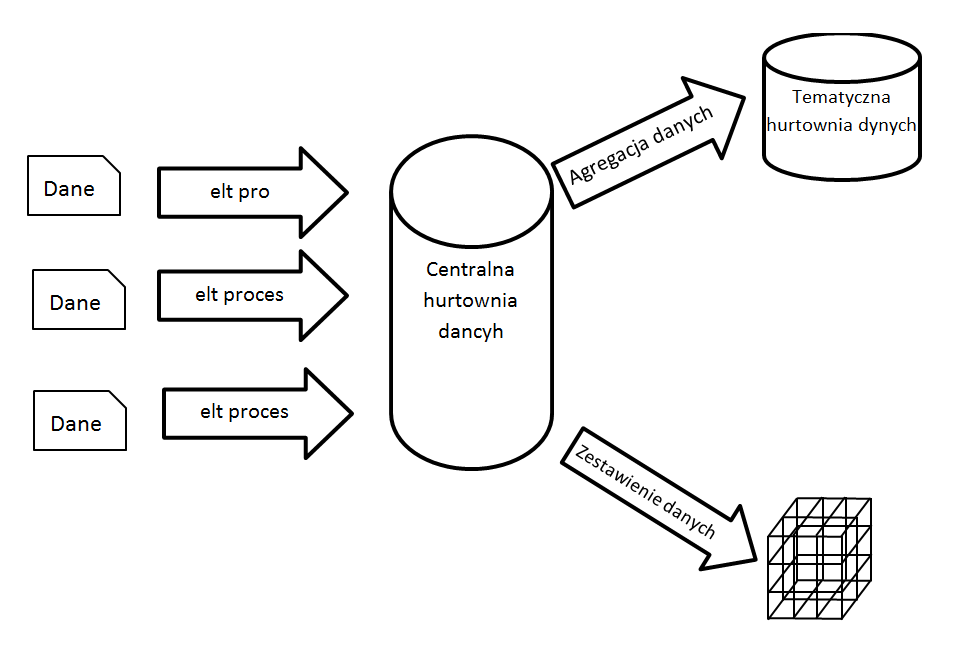
\includegraphics[width=0.7\textwidth]{AHD.png}
  \end{center}
 \caption{Architektura hurtowni danych. }
    \label{fig:AHD}
\end{figure}
\end{center}


Strukturę przepływu danych możemy podzielić na:
\begin{itemize}
 \item \textbf{Źródło danych \ang{source} } --- 
        są to dane, które będą pobierane do hurtowni danych 
 \item \textbf{proces ETL \ang{extract, transfer, load} } --- 
    procesem elt nazywamy czynności wykonywane w celu pobrania danych źródłowych
    przekształcenie w odpowiedni format danych, a następnie umieszczeni ich w centralnej hurtowni danych,
    proces elt dokładnie będzie omówiony w rozdziale drugim.
 \item \textbf{centralna hurtownia danych \ang{center data  warehouse}} --- 
    jest to miejsce docelowe przetowrzonych danyc ze źródeł,						                                          
 \item \textbf{hurtownie tematyczne \ang{data marts}} --- 
    zawierają wybrane dane z centralnej hurtowni danych w~sposób 
    zagregowany, umożliwiające szybkie operowanie sporządzanie raportów,
 \item \textbf{zestawienie danych } --- 
    docelowym produktem hurtowni danych jest tworzenie odpowiednich zestawień danych.
    Na rysunku \ref{fig:AHD}, został przedstawiona jako kostka.
\end{itemize}

 
Tworzenie hurtowni danych jest stosunkowo młodą dziedziną, która się dynamicznie rozwija.
Dzięki zastosowaniom CRM odniosły one sukces co spowodowało większe zapotrzebowanie na przechowywanie
 i~analizowanie danych historycznych. Przedstawiona architektura danych na rysunku \ref{fig:AHD}, 
 nie spełnia swojej roli dla Hurtowni Danych, w których przyrost  danych jest bardzo duży.
Poniżej została przedstawione inna architektura danych.
\begin{center}
\begin{figure}[H]
  \begin{center}
    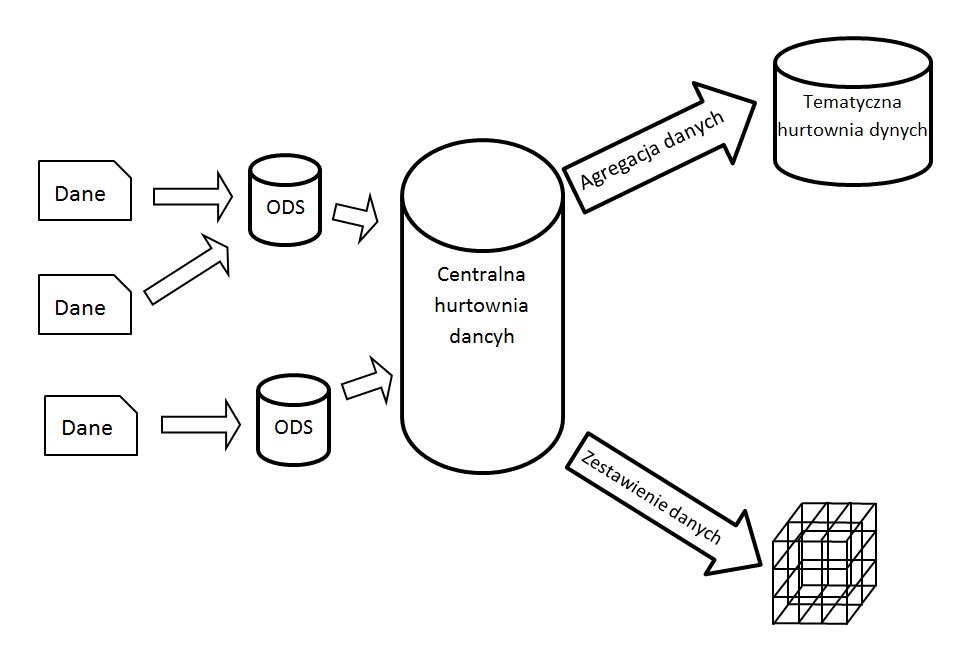
\includegraphics[width=0.7\textwidth]{AHD_ODS.png}
  \end{center}
  \caption{Architektura hurtowni danych z magazynem danych ODS. }
    \label{fig:ODS}
\end{figure}
\end{center}

Do architektury z rysunku \ref{fig:AHD} został dodany magazyn danych operacyjnych \ang{operational data store, ODS}, który
pełni role magazynu danych. Ładowane są do niej dane pobrane ze źródeł i przetworzone w celu uzyskania zgodności typów danych.
Kolejnym etapem jest załadowanie danych w sposób zagregowany do centralnej hurtowni danych.


\section{Projektowanie hurtowni danych.}
Projektowanie hurtowni danych tak jak relacyjnych baz danych polega na utworzeniu następujących modeli:

\begin{itemize}
 \item \textbf{Model pojęciowy} --- 
    przy użyciu języka biznesowego w danej firmie opisuje się cele biznesowe, 
     które będzie można określić przez gromadzenie ściśle określonych danych.
    Na modelu pojęciowym powinny, być zaznaczone nazwy kolumn, które mają być przechowywane 
      w tabeli znajdującej się w Hurtowni Danych
 \item \textbf{Model logiczny} --- 
    jest to opis elementów  logicznych hurtowni danych, wykonany np. w języku UML.
 \item \textbf{Model fizyczny} --- 
    jest to opis indeksowania, partycjonowania, opis sprzętu komputerowego, sieci
     rozmieszczenie poszczególnych zasobów fizycznych.
\end{itemize}

% Do tworzenie modelu logicznego najczęściej wykorzystywane
% są schematy logiczne (podział na tablicy): gwiazda i płatek śniegu. Zostały one zaprezentowane 
% w podrozdziałach.

Najpopularniejszymi metodami przyjętymi podczas tworzenia hurtowni danych są:
\begin{itemize}
 \item \textbf{Projektowanie wstępujące} (od szczegółu do ogółu)---
    polega na tworzeniu wszystkich etapów hurtowni danych 
     jednocześnie, a następnie na integracji poszczególnych etapów ze sobą.
 \item \textbf{Projektowanie zstępujące} ---
    Dopóki jeden etap tworzenia hurtowni danych się nie skończy, 
     to następny się nie zacznie. Jeżeli pojawią się błędy to wraca się do poprzedniego etapu i zaczyna się prace 
     na kolejnym etapie od nowa.
\end{itemize}



\section{Wielowymiarowy danych danych}
Wielowymiarowym modelem danych \ang{Multidimensional Data Model} 
nazywamy dane zorganizowane w:
\begin{itemize}
 \item 
    \textbf{fakt \ang{facts}  } ---   są to dane opisujące jakieść zdarzenie, 
    tabelkę przechowującą te dane nazywamy  \textit{tablicą faktów} 
    Fakt opisany jest przez wymiary i miary,
 \item \textbf{wymiar \ang{dimension}} --- 
    Jest jakąś cechą opisującą dany fakt, cechy te znajdują się w tablicy wymiarów i są opisane przez atrybuty,
 \item \textbf{atrybut} \ang{ attribute}  --- 
    Przechowuje dodatkowe informację na temat wymiaru,
 \item \textbf{miara \ang{measures}} --- 
    Jest wartością mierzalną przypisaną do pojedynczego rekordu w tablicy faktów. 
\end{itemize}

Model ten jest zintegrowaną częścią z systemem OLAP.
Podstawowym atutem wielowymiarowego modelu danych jest proste zrozumienie hurtowni danych 
 i poruszania się po niej w sposób efektywny, szybsze wykonywanie zapytań zadawanych do hurtowni danych, 
 Jak również możliwość analizy danych w różnych wymiarach, 
które jest bardzo istotne ze względów biznesowych:
\begin{itemize}
 \item Oglądanie informacji rozłożonych w czasie,
 \item Wyświetlanie informacji w sposób graficzny,
 \item Możliwość zmiany przekroju danych w dowolny sposób,
 \item Analizę danych pod kątem informacji istotnych dla danej firmy.
\end{itemize}

Podstawowymi schematami wielowymiarowego modelu danych są:
\begin{itemize}
 \item schemat gwiazdy \ang{Star schema} 
 \item schemat płatka śniegu \ang{Snowflake schema}
\end{itemize}

\subsection{Schemat gwiazdy}
Schemat gwiazdy jest podstawowym schematem wielowymiarowego modelu danych,
 w którym znajduje się jedna tabela faktów połączona z wieloma tabelami wymiarów.
Tabela faktów w tym schemacie jest w trzeciej postaci normalnej, a tabela wymiarów jest w drugiej postaci normalnej,
dzięki takiej strukturze możliwe jest szybsze przeglądanie danych poprzez:
\begin{itemize}
 \item poszczególne wymiary,
 \item sumowanie danych,
 \item agregację danych,
 \item filtrowanie danych
\end{itemize}

Na rysunku  \ref{fig:gwiazda} został przedstawiona przykładowa architektura schematu gwiazdy.
\begin{center}
\begin{figure}[H]
  \begin{center}
    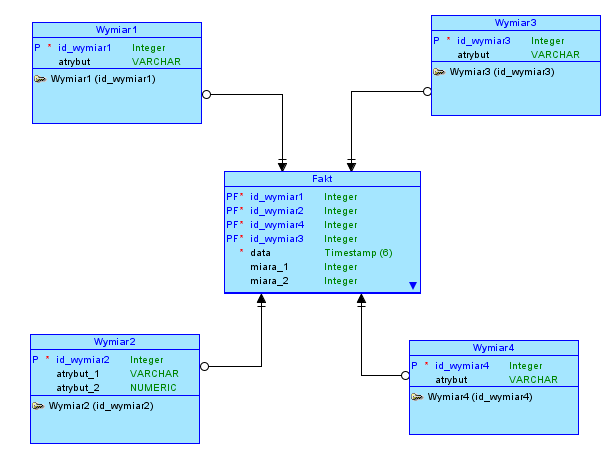
\includegraphics[width=0.7\textwidth]{gwiazda.png}
  \end{center}
  \caption{Przykładowy schemat gwiazdy w postaci abstrakcyjnej. }
    \label{fig:gwiazda}
\end{figure}
\end{center}
Poniżej znajduje się listing zapytań do bazy danych w języku postgresql,
 który realizuje model logiczny gwiazdy zawarty na rysunku \ref{fig:gwiazda}
\lstinputlisting[language=sql, caption = {Listing kodu tworzący schemat gwiazdy. } ]{"./sql/gwiazda.sql"}
\subsection{Schemat płatka śniegu}
Architektura schematu gwiazdy jest uproszczoną formą architektury płatka śniegu.
Podstawową różnicą pomiędzy tymi schematami jest tabela wymiarów, która jest znormalizowana.

Schemat płatka śniegu jest stosowany wtedy, gdy tabela wymiarów osiąga duży rozmiar.
Normalizuję się tabele wymiarów, aby zmniejszyć jej liczebność, dzięki czemu czas zapytań, 
powinien się znacząco skrócić. 
Wadą tego podejścia jest, że im bardziej znormalizowana jest tabela wymiarów,  
to tym bardziej skomplikowane łączenia SQL muszę zostać użyte, aby pobrać odpowiednie
dane z hurtowni danych. \cite{cube}

Przykładowa architektura płatka śniegu został przedstawiona na rysunku \ref{fig:platek_sniegu} .

\begin{center}
\begin{figure}[H]
  \begin{center}
    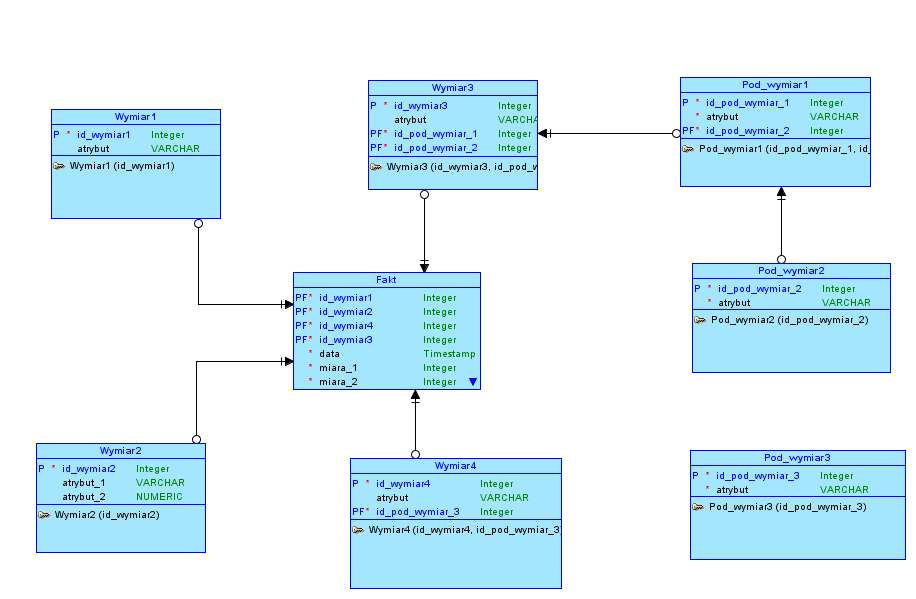
\includegraphics[width=0.7\textwidth]{platek_sniegu.png}
  \end{center}
  \caption{Przykładowy schemat płatka śniegu w postaci abstrakcyjnej. }
    \label{fig:platek_sniegu}
\end{figure}
\end{center}







\begin{comment}
 
\end{comment}
